\documentclass[UTF8,9pt]{ctexart}
\usepackage{amsfonts}
\usepackage{geometry}
%\usepackage[T1]{fontenc}                                             %change font
\usepackage{mathtools}                                                %align needed
\usepackage{balance}                                                  %blance when there two columns
%\usepackage{txfonts}                                                  %面积分体积分
\usepackage{bm}                                                       %bold font
\usepackage{mathrsfs}                                                 %change greek font style
\usepackage{enumerate}                                                %Sort by number
\usepackage{supertabular}                                             %allow long table in 2 pages
\usepackage{soul}                                                     %highlight using \hl
\usepackage{fontspec}                                                 %expand font type
\usepackage{graphicx}                                                 %to input pictures
\usepackage[colorlinks,linkcolor=red,anchorcolor=blue,citecolor=green]{hyperref}                                                %cite
\usepackage{verbatim}                                                 %comment                            
\usepackage{multicol}
%begin{newcommands}
    \newcommand\qqed{\rightline{$\square$}\\ }                                 %\square,QED
    \newcommand\norm[1]{\left\| #1 \right\|}                                 %|| ||
    \newcommand\s{\sqrt} 
    \newcommand\cm{\mathscr}                                               %dbar
    \newcommand\dbar{\text{\dj}}                                           %dbar
    \renewcommand\d{\mathop{}\!\mathrm{d}}                                            %d
    \newcommand\sch{Schrödinger}                                           %Schrödinger
    \newcommand{\dd}[3][]{\frac{\mathrm{d}^{#1} #2}{\mathrm{d} {#3}^{#1}}}   %d/d^n
    \newcommand{\dt}[2][]{\frac{\mathrm{d}^{#1} #2}{\mathrm{d} t^{#1}}}    %d/dt^n
    \newcommand{\pp}[3][]{\frac{\partial^{#1} #2}{\partial {#3}^{#1}}}       %∂/∂^n
    \newcommand{\pt}[2][]{\frac{\partial^{#1} #2}{\partial t^{#1}}}        %∂/∂t^n 
    \newcommand{\f}[2]{\frac{#1}{#2}}                                      %A/B
    \newcommand{\ff}[1]{\frac{1}{#1}}                                      %1/A
    \newcommand\rank{\operatorname{rank}}                                        %rank
    \newcommand\tr{\operatorname{tr}}                                            %tr
    \newcommand\e[1]{\times 10^{#1}}                                       %×10^
    \newcommand\mo{^{-1}}                                       %^{-1}
    \renewcommand\Re{\operatorname{Re}}                                          %Re
    \renewcommand\Im{\operatorname{Im}}                                          %Im
    \renewcommand\ln{\operatorname{ln}}                                          %ln
    \newcommand\Ln{\operatorname{Ln}}                                            %Ln
    \renewcommand\arg{\operatorname{arg}}                                  %arg
    \newcommand\ip{\implies}                                               %→
    \newcommand\tm{\times}                                                 %×
    \renewcommand\l{\lambda}                                               %λ
    \renewcommand\a{\alpha}                                                %α
    \renewcommand\b{\beta}                                                 %β
    \renewcommand\C{\bm{Const}}                                            %Const
    \newcommand\D{\Delta}                                                  %Δ
    \newcommand\de{\delta}                                                 %δ
    \newcommand\ep{\varepsilon}                                            %ε
    \newcommand\g{\gamma}                                                  %γ
    \renewcommand\k{\kappa}                                                %κ
    \newcommand\n{\nabla}                                                  %nabla
    \newcommand\laplace{\nabla^2}                                          %laplace
    \newcommand\grad{\nabla}                                               %grad
    \renewcommand\div{\nabla\cdot}                                         %div
    \newcommand\curl{\nabla\times}                                         %\nabla\times
    \renewcommand\o{\omega}                                                %ω
    \newcommand\sg{\sigma}                                                 %σ
    \newcommand\p{\phi}                                                    %phi
    \newcommand\vp{\varphi}                                                %phi
    \renewcommand\t{\theta}                                                %$\t$
    \newcommand\abs[1]{\left| #1 \right|}                                  %|A|
    \renewcommand\exp{\operatorname{exp}}                                  %exp
    \newcommand\se{\section}                                               %section
    \newcommand\sub{\subsection}                                           %subsection
    \newcommand\dis{\displaystyle}                                         %big equation
    \AtBeginDocument{\renewcommand{\bar}{\overline}}                       %bar
    \AtBeginDocument{\renewcommand{\hat}{\widehat}}                        %hat
    \renewcommand{\arraystretch}{1.2}                                      %change array stretch
    \newcommand\ca{\frac{1}{4\pi\varepsilon_0}}                                 %constA
    \newcommand{\ar}[2][rl]{\begin{array}{#1}                              %begin an array
            #2
        \end{array}}                                                 
    \newcommand\bkt[1]{\left< #1 \right>}                                  %<x>
    \newcommand\putfig[2]{                                                 %put a figure
        \begin{center}    
            \includegraphics[scale=#1]{#2}
        \end{center}}
    \newcommand{\rk}[1]{\begin{enumerate}                              %enumerate
        #1
    \end{enumerate}}                                             

%end{newcommands} 
\setlength\columnseprule{0.4pt}
%\allowdisplaybreaks[4]                                                %allow page change in a table/align
\linespread{1.5}                                                      %change line spread
\setlength{\arraycolsep}{5pt}                                           %space after &
\author{肖涵薄 31360164}
\usepackage[version=3]{mhchem}
\title{“在生活中感知材料魅力”材料通识课习题} 
\begin{document} 
\maketitle
\se{什么是锂离子电池?列举1种典型的锂离子电池体系并描述其原理。}
\sub{锂离子电池介绍}
锂离子电池是一种依靠锂离子在正负极之间来回移动产生电能的电池。与传统电池技术相比,锂离子电池充电更快,而且更高的功率密度可实现更长的电池使用时间,具有高能量密度,无记忆效应,在不使用时只有缓慢电荷损失。同时更加轻巧。其能量密度可达150~200Wh/kg\cite{2},开路电压高达3.3~4.2V,且解决了以前电池有记忆效应导致对充放电时机要求严格的缺点。但同时也有不耐受过充放,衰老怕热等缺点。

锂离子电池的电解液现在通常为凝胶体或聚合物 (即聚合物锂离子电池)制成。由于目前尚未发现能够在室温下有效运送锂离子的聚合物,所以大多数的“塑胶封袋”锂离子/锂聚合物电池事实上都是结合凝胶体和聚合物的混合型电池。
\sub{LFP电池}
目前主流的商业产品中,锂离子电池的正极通常选择\ce{LiFePO4},负极通常选择石墨。下面描述这种比较主流的电池的原理:
\begin{itemize}
    \item 正极采用\ce{LiFePO4}的锂离子电池称为磷酸铁锂电池 (LFP),相较于钴锂、镍锂等其他锂电池方案,同时拥有他们的主要优点且不含钴这样的贵重元素。而且工作电压适中,电容量大。1C充放循环寿命可做到2000次,穿刺不爆炸,过充时不容易燃烧和爆炸。是目前产业界认为较符合环保、安全和高性能要求的锂离子电池。
    \item 安全性能高\\
    磷酸铁锂电池较高的安全性来自于磷酸铁锂晶体中稳固的\ce{P-O}键。如图\ref{s},磷酸根中的磷与四个氧原子形成以磷为中心共边的四面体\ce{PO4},借由铁的\ce{FeO6}八面体和磷的\ce{PO4}四面体所构成的空间骨架,使得材料本身具有良好的热稳定性和循环性能。 

    \begin{figure}[htbp]
        \centering
        
\includegraphics[scale=0.05]{1.png}
        \caption{磷酸铁锂分子结构式}\label{s}
    \end{figure}

    \begin{table}[ht]
        \centering
        \begin{tabular}{|c|c|c|}
        \hline
        正极材料      & 平均输出电压 & 能量密度      \\ \hline
        \ce{LiCoO2}    & 3.7 V  & 140 mAh/g \\ \hline
        \ce{Li2Mn2O4}  & 3.7 V  & 100 mAh/g \\ \hline
        \ce{LiFePO4}   & 3.3 V  & 100 mAh/g \\ \hline
        \ce{Li2FePO4F} & 3.6 V  & 115 mAh/g \\ \hline
        \end{tabular}
        \caption{不同的正极材料对照}\label{1}
    \end{table}   

    \item 性能缺陷\\
    磷酸锂铁虽然得到了产业界的认可,但仍然具有提升空间。表\ref{1}为各类正极材料的电压和能量密度,可以看到其他几种正极材料虽然不具备磷酸铁锂原料丰富,安全等优点,但输出电压和能量密度均更高。这是磷酸铁锂振实密度与压实密度很低导致的。即使将其纳米化和碳包覆也没有解决这一问题。
    \item 反应机理\\
    \ce{LiFePO4}电池的内部是橄榄石结构的\ce{LiFePO4}作为电池的正极,由铝箔与电池正极连接,中间是聚合物的隔膜,它把正极与负极隔开,但锂离子\ce{Li+}可以通过而电子\ce{e-}不能通过,右边是由碳(石墨)组成的电池负极,由铜箔与电池的负极连接。电池的上下端之间是电池的电解质,电池由金属外壳密闭封装。
    \ce{LiFePO4}电池在充电时,正极中的锂离子\ce{Li+}通过聚合物隔膜向负极迁移;在放电过程中,负极中的锂离子\ce{Li+}通过隔膜向正极迁移。锂离子电池就是因锂离子在充放电时来回迁移而命名的。一般来讲,\ce{LiFePO4}电池的标称电压是3.2V、终止充电电压是3.6V、终止放电压是2.0V。
    \item 正极反应: 放电时锂离子嵌入,充电时锂离子脱嵌 (锂离子进入正极材料的过程叫“嵌入”,离开的过程叫“脱嵌”)。\\
    充电时: \ce{LiFePO4 -> Li_{1-x}FePO4 + xLi+ + xe-}\\
    放电时: \ce{Li_{1-x}FePO4 + xLi+ + xe- -> LiFePO4}
    \item 负极反应: 放电时锂离子脱插,充电时锂离子插入(锂离子进入负极材料的过程叫“插入”,离开的过程叫“脱插”)。\\
    充电时: \ce{xLi+ + xe- + 6C -> Li_xC6}\\
    放电时: \ce{LixC6 -> xLi+ + xe- + 6C}

    \begin{figure}[htbp]
        \centering
        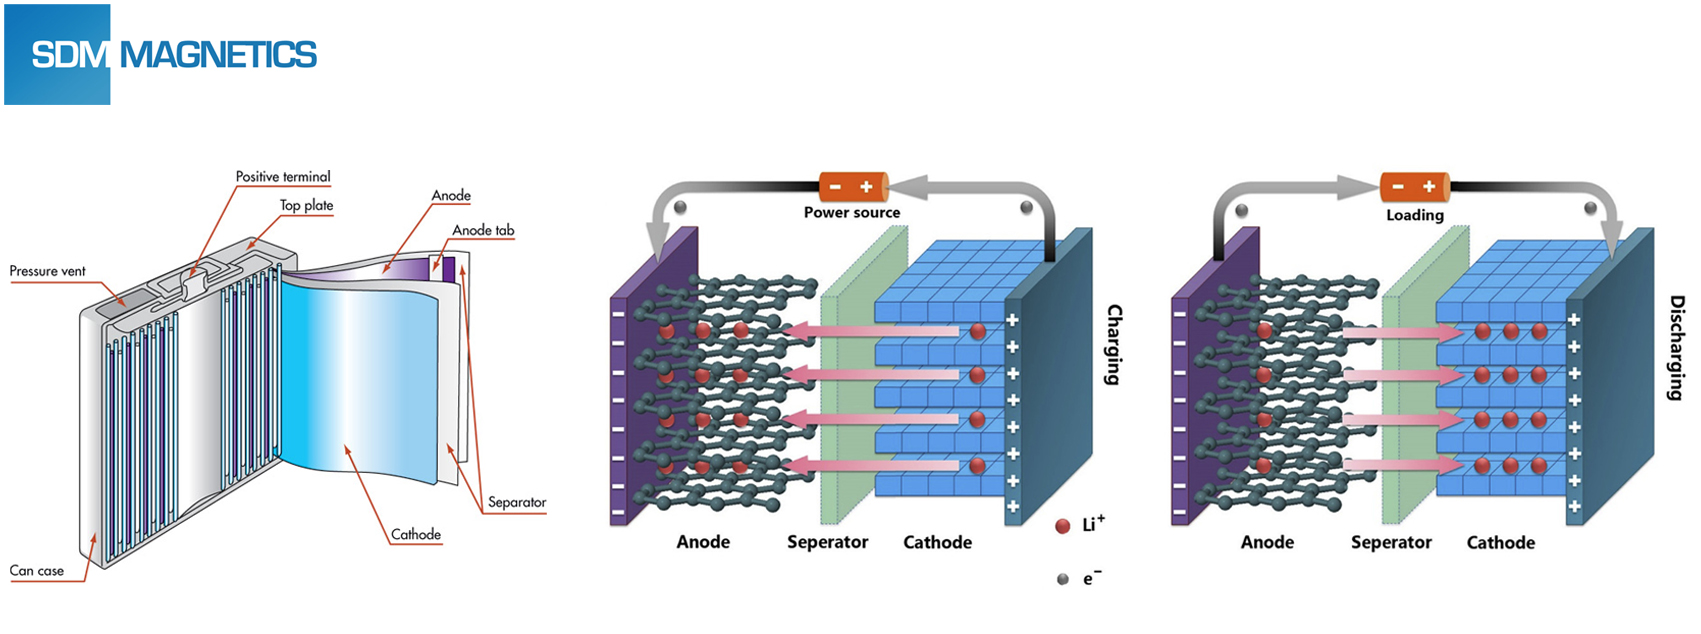
\includegraphics[scale=0.2]{1-45.jpg}
        \caption{锂电池充放电反应示意图}
    \end{figure}

    \item 电解质溶液\\
    溶质通常选择锂盐。如高氯酸锂(\ce{LiClO4})、六氟磷酸锂(\ce{LiPF6})、四氟硼酸锂(\ce{LiBF4})。
    由于电池工作时水会电解,因此需要采取有机溶剂,有机溶剂常常在充电时破坏石墨的结构,导致其剥脱,并在其表面形成固体电解质膜导致电极钝化。有机溶剂还带来易燃、易爆等安全性问题。
\end{itemize}
\se{有哪些主要的碳材料,石墨烯的主要特点是什么?有哪些主要的应用?}
\sub{主要的碳材料}
主要的碳材料包括富勒烯、碳纳米管、碳纤维、石墨烯等新型纳米碳材料和传统的金刚石、石墨等材料。其中,富勒烯为零维材料,碳纳米管、碳纤维属于一维材料,石墨烯属于二维材料,除此以外还有以金刚石为代表的三维材料和无定型碳等无定型材料。

\begin{figure}[htbp]
    \centering
    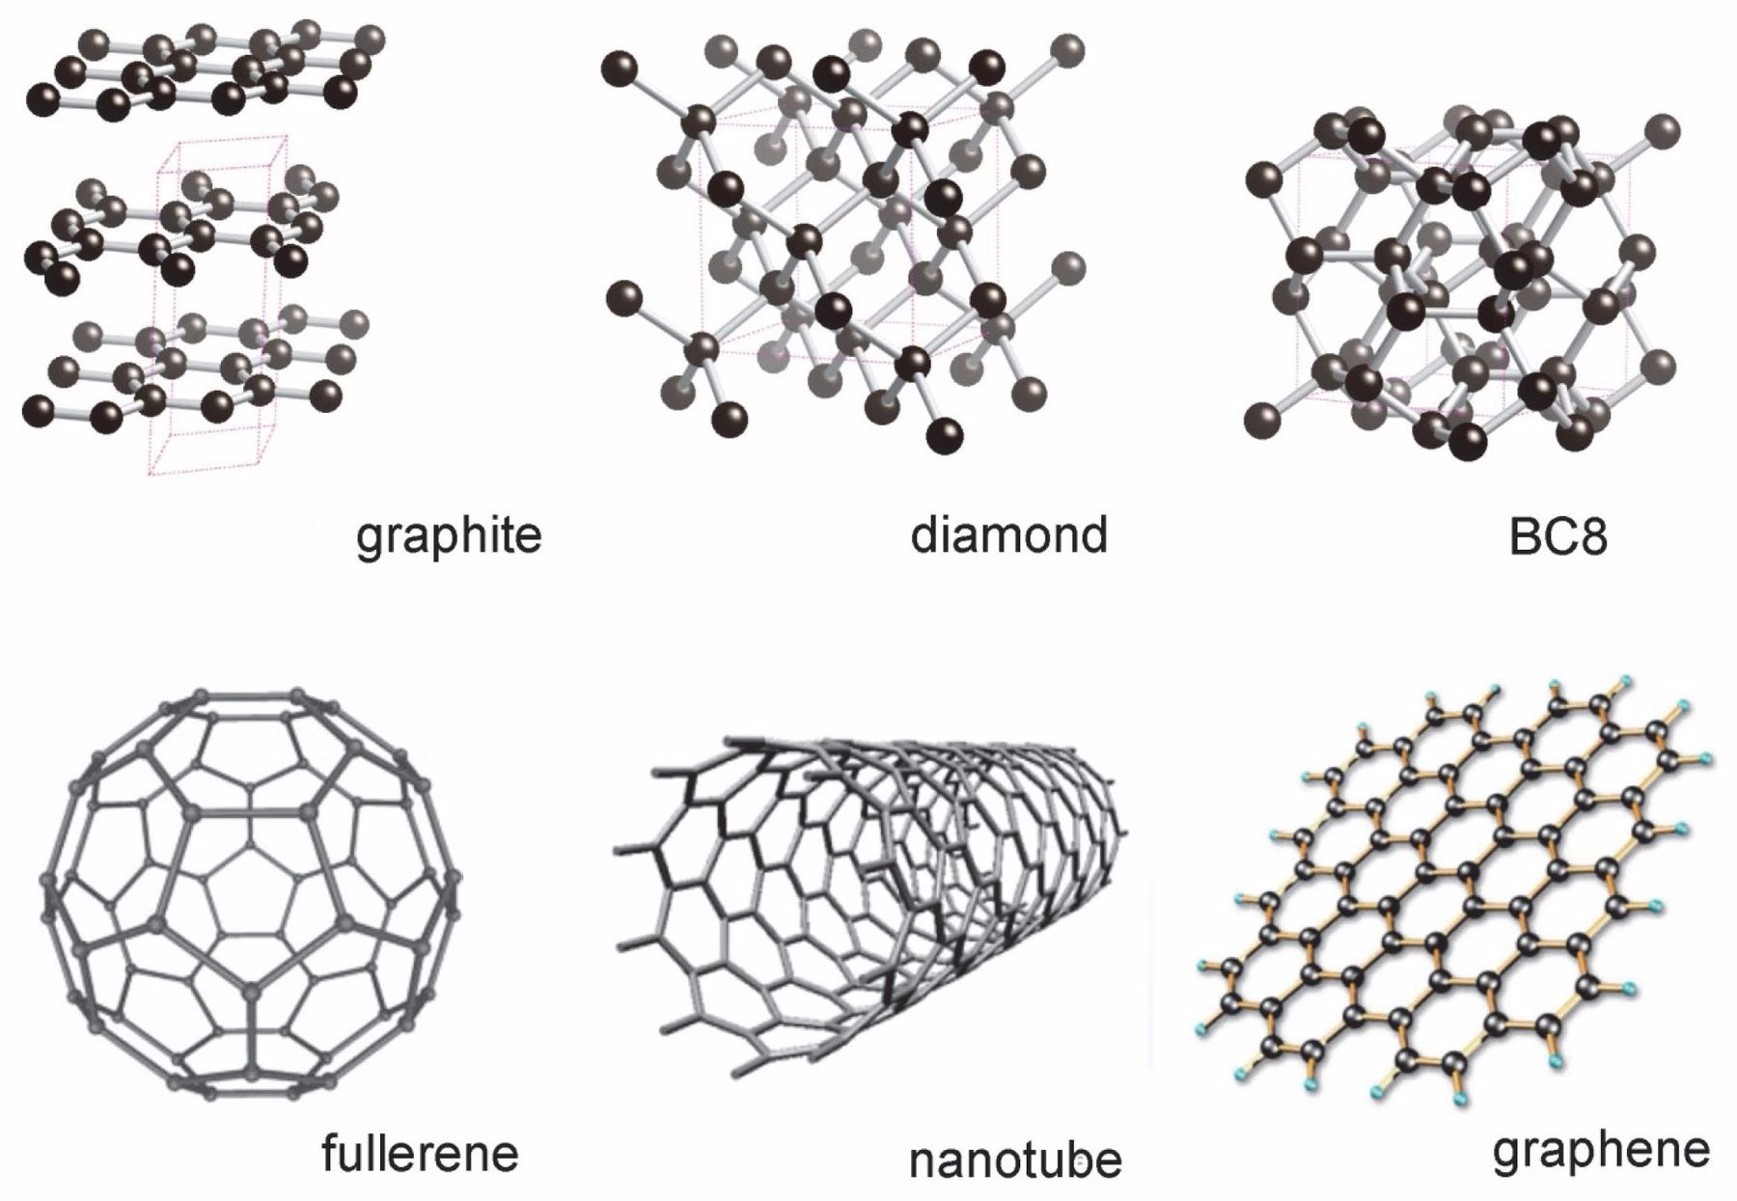
\includegraphics[scale=0.2]{2.jpg}
    \caption{各类纳米碳材料}
\end{figure}

它们不同的维度主要来自于形成\ce{C-C}键时的杂化方式。以sp杂化时,键角为$180^{\circ}$,易形成一维链式结构,以\ce{sp^2}杂化时,键角为$120^{\circ}$,易形成二维平面,而以\ce{sp^3}杂化时,形成空间四面体结构,会形成空间网状结构。
\sub{石墨烯的特点}
石墨烯是一种由碳原子以\ce{sp^2}杂化轨道组成六角型呈蜂巢晶格的平面薄膜,只有一个碳原子厚度的二维材料。石墨烯目前是世上最薄却也是最坚硬的纳米材料,它几乎是完全透明的,只吸收2.3\%的光;导热系数高达5300 W/m·K,高于纳米碳管和金刚石,常温下其电子迁移率超过15000 cm${}^2$/V·s,又比纳米碳管或硅晶体高,而电阻率只约$10^{-6}$ Ω·cm,比铜或银更低,为目前世上电阻率最小的材料。由于它的电阻率极低,电子的移动速度极快,因此被期待可用来发展出更薄、导电速度更快的新一代电子元件或晶体管。石墨烯实质上是一种透明、良好的导体,也适合用来制造透明触控萤幕、光板、甚至是太阳能电池。

在石墨烯出现之前,凝聚态物理有一个Mermin-Wagner 定理,``任何具有连续对称性的二维热力学系统,在非零温下,其连续对称性不可能发生自发破缺。''而对二维晶体做法向平移,系统状态会发生改变,也就是说二维晶体是不能存在的。当时的物理学家认为,虽然现实中不存在严格的二维晶体,但即使是准二维的晶体,也应该只能在接近绝对零度的时候才能出现一样 (就像超导)。而单层石墨烯在室温就能制备否定了这一观点。现在对这一现象有许多解释,例如石墨烯有纳米级的起伏,即使离准二维也相差很远,以及石墨烯有衬底,这不满足定理要求的无外场的条件。

量子霍尔效应只发生于二维导体,石墨烯有整数量子效应,它的霍尔电导为量子电导的奇数倍,对这个现象的解释是``电子在石墨烯里遵守相对论量子力学,没有静质量''。后来,在2007年前后又进一步的观测到了石墨烯的分数量子霍尔效应。且将石墨烯置于外磁场中时,还会产生反常霍尔效应,其$\sg$的阶梯序列同时发生平移和分裂。

电子传输测量结果显示,在室温状况,石墨烯具有惊人的高电子迁移率,其数值超过15000 \ce{cm^2V^{−1}s^{−1}}。其电阻率最低能到达$10^{-8}$ Ω·cm,小于银$1.59 \e{-6}$ Ω·cm的电阻率,因此石墨烯是非常优良的导体。
\sub{应用}
\rk{
    \item 石墨烯电池。\\不久前西班牙一家以工业规模生产石墨烯的Graphenano公司同西班牙科尔瓦多大学合作开发出首例石墨烯聚合材料电池,其储电量是目前市场最好产品的三倍,用此电池提供电力的电动车最多能行驶1000公里,而其充电时间不到8分钟。电池技术是电动汽车大力推广和发展的最大瓶颈,石墨烯储能器件研制成功后,若能批量生产,则将为电池产业乃至电动车产业带来新的变革。
    \item 透明电极。\\传统电导电极用的是氧化铟锡,而这种材料脆度较高,比较容易损毁。透光率也比较低。与之相比,石墨烯具有极高的电导率,未来可能用来制造更薄的电子元件或晶体管,而且透光率非常高,也适合用来制造透明触摸屏。不仅更加坚硬,性能也更好。
    \item 集成电路芯片。\\由于硅导电性能不佳,现在的集成电路发热情况难以解决,而石墨烯与碳纳米管这对亲兄弟具有类似的性能,高的载流子迁移率以及热导,都成为了下一代集成电路芯片材料的候补对象。2012年,美国IBM公司成功研制出首款由石墨烯圆片制成的集成电路,使得石墨烯特殊的电学性能彰显出应用前景。
    \item 新能源电池。\\石墨烯太阳能技术的光电转换效率高达60\%,是现有多晶硅太阳能技术的2倍。之前美国麻省理工学院已成功研制出表面附有石墨烯纳米涂层的柔性光伏电池板,可极大降低制造透明可弯曲太阳能电池的成本。 
    \item 超级电容器。\\美国加州大学洛杉矶分校的研究人员开发出一种以石墨烯为基础的微型超级电容器,该电容器不仅外形小巧,而且充电速度为普通电池的1000倍。这种超级电容器的储存能量密度会大于现有的电容器。
}
\se{什么是仿生材料学?列举1种仿生材料及其应用。}
\sub{仿生材料学概观}
仿生材料指模仿生物的各种特点或特性而开发的材料。人工制造的结构物同自然界各种的结构物相比较,有很多可以改进的地方,仿生材料学受生物结构和功能的启发,通过研究生物体宏观、微观多尺度结构与其特性之间的相关性,设计合成具有该特性的物质和结构,最终得到具备特定功能的新材料。仿生这一思想早已出现并应用于人类的生产生活,例如上课时提到的各种模仿荷叶的超疏水材料,同学演讲时提到的模仿蜘蛛丝的高强度材料,模仿壁虎的粘胶等。经过长期的演化和自然选择,生物系统通过优化其组织结构及界面性质等方法,最终进化出了能够响应外界刺激、适应环境变化的优异性能。现代化表征及制备合成技术的高速发展推动了人类对这些优异生物特性的深入认知,得益于此,自然宏观现象背后的微观作用机制为新材料的研发带来了更多的设计灵感。

自然界的生物体给人类带来了无尽的设计灵感,其中包括了仿生材料领域的诸多研究热点,例如仿生定向输运材料、仿生超疏水材料、仿生高黏附材料、仿生轻质高强度材料、仿生智能薄膜材料等。
\sub{仿生材料在液流电池的应用}
液流电池是一种二次燃料电池,其中含有一种或多种溶解的电活性元素的电解质流过电化电池,通过更换电解液(以与内燃机的再填充燃料箱类似的方式)可以快速“再充电”液流电池,同时回收用过的材料以重新通电。因此,液流电池在大规模储能领域应用广泛,并被广为研究。同时,液流电池也不可避免地存在一些问题。其中一个关键问题在于,用于储存能量的水溶性有机分子水溶性差,或者不稳定,往往难以实现其理论容量,导致液流电池的功能难以最大程度实现。

鉴于此,2018年Nature Energy上一篇文章通过仿生改性的吩嗪衍生物作为水性有机液流电池的负极电解液,其可逆容量达到理论容量的90\%。

\begin{figure}[htbp]
    \centering
    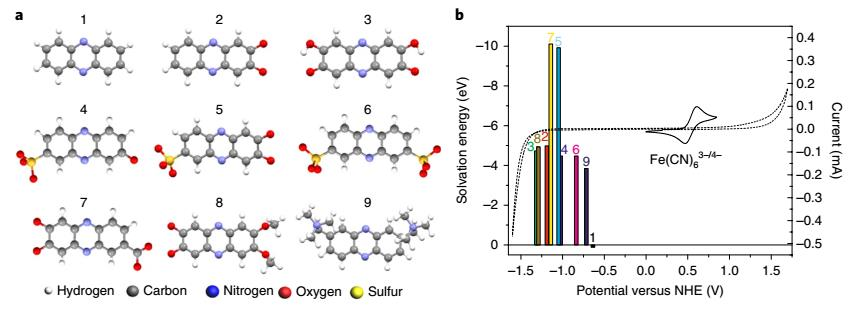
\includegraphics[scale=0.4]{3.jpg}
    \caption{吩嗪衍生物分子结构和计算预测的性能}
\end{figure}

在生物系统的产甲烷古细菌群中,吩嗪类材料常常被用于氧化还原媒介。基于生物启发,研究人员用几乎不溶于水的杂环吩嗪材料为研究对象合成得到仿生的改性吩嗪材料(7,8-dihydroxyphenazine-2-sulfonic acid,DHPS),使其溶解度增加到1.8 M(电子摩尔浓度2.8M),氧化还原电位位移超过400 mV。在接近其饱和浓度的条件下,可逆容量达到67 Ah \ce{l^{-1}}(1.4 V),循环500次后容量保持率为99.98\%,相当于每循环一次,容量损失仅有0.0195\%。

\begin{figure}[htbp]
    \centering
    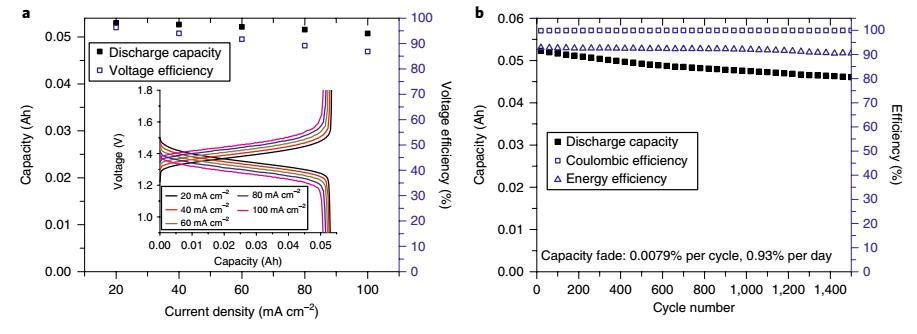
\includegraphics[scale=0.4]{4.jpg}
    \caption{低浓度流体电池性能}
\end{figure}

这项研究提供了新的水溶性有机分子,将水溶性液流电池的容量推到了极限,为开发更大容量的实用性液流电池提供了借鉴。
\se{贝壳是一种典型的有机--无机复合材料,具有特殊的结构并赋予其优良的力学性能,请进行具体描述。}
\sub{贝壳的结构和成分}
贝壳是软体动物在环境温度与压力下将周围环境中的无机矿物(\ce{CaCO3})与自身生成的有机物相结合制造出的复合材料,贝壳的形成过程是一种生物矿化过程。贝壳根据形成的方式和组成结构不同分为3层。最外层为角质层,是硬蛋白质的一种,能耐酸的腐蚀;中间的棱柱壳层,它占据壳的大部分,由角柱状的方解石构成,角质层和棱柱层只能由外套膜背面边缘分泌而成;内层为珍珠层,也由角柱状方解石构成,它由外套膜的全表面分泌形成,并随着贝类的生长而增厚,富有光泽。贝壳虽然种类繁多,形态各异,颜色不同,但化学组成相似,主要有占全壳95\% 的碳酸钙和少量的贝壳素。

贝壳中的有机基质一般仅占壳重的0.3\%-5\%,通常可分为5层。其中心是由两层富含Gly和Ala的疏水性蛋白质夹一薄层卜几丁质所构成,疏水核心两侧为富含ASp和Gill的亲水性蛋白质,与矿物相紧密相连。通常根据溶解性将其分为可溶性有机基质(SM)和不溶性有机基质(IM)。SM在晶体的成核、定向、生长、形态控制等方面起调控作用,同时可能还具有控制离子运输的功能;而IM则主要作为生物矿化的构架蛋白,为晶体的核化、生长提供结构支撑。

 一般认为贝壳特殊的结构主要来自于其珍珠层。对贝壳珍珠层
的形成过程比较成熟的理论认为:首先由细胞分泌的有机质自组装成层状隔室,每一层有机质上有纳米级小孔,导致上下层隔室相通。然后,在有机/无机间的分子识别作用下(贝壳生物矿化过程是生物有机大分子指导无机晶体的晶核形成、定向、形态及晶体生长动力学的过程。有机大分子对无机晶体的控制作用是一个相当复杂的过程,目前一般将这种作用称为分子识别。),文石晶体从最下面一层有机质上开始定向成核,并往外生长。由于隔室相通,下一层隔室长满之后可通过小孔继续往上一层隔室中生长,而小孔可以保证所需要的离子的运输。因此上一层的晶体填充不需要重新成核,从而保证了珍珠层中每一层的文石晶体具有一致的取相,又保证了文石层和有机层交替堆叠,从而使珍珠层具有优异的力学性能。其生长示意图见图\ref{bk}.

\begin{figure}[htbp]
    \centering
    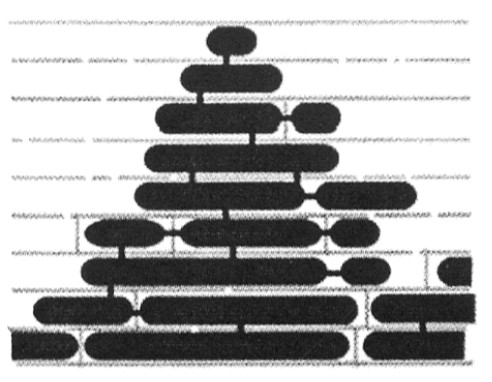
\includegraphics[scale=0.4]{6.jpg}
    \caption{贝壳矿化时文石晶体在预先自组装形成的有机基质片(糖,蛋白质)隔室中的成核和生长}
    \label{bk}
\end{figure}

根据研究结果,珍珠层优异力学特性主要来源于以下因素:
\rk{
    \item 裂纹偏转及纤维拔出的作用。\\
    当珍珠层沿垂直文石层面断裂时,由于有机基质的强度相对较弱,在有机/无机界面上易于诱导产生裂纹的频繁偏转,造成裂纹扩展路径的增长,从而使裂纹扩展过程吸收了更多的能量,而且导致裂纹从应力有利状态转为不利状态,增大了扩展的阻力,提高了材料的韧性。
    \item 有机基质的桥连作用。\\
    约占贝壳重量5\%的有机大分子使本质上各向异性的矿物质自组装成各向同性的纳米结构体,其在贝壳增韧机制中起到了不可替代的作用。珍珠层发生变形与断裂时,文石层间的有机基质发生塑性变形并且与相邻晶片粘结良好。
    \item 矿物桥的作用。\\
    在珍珠层的断裂过程中,由于矿物桥的存在及其位置的随机性,加强了裂纹扩展的偏转作用;在裂纹穿过有机基质后,由于有机基质和矿物桥的作用,上下文石片间仍然保持着紧密连接,除有机相和文石间的结合力和摩擦力将阻止晶片的拔出外,要拔出晶片必须先“剪断”晶片上所有的矿物桥;此外,有机基质与文石晶片的紧密结合既保护了矿物桥,又和矿物桥共同阻止了晶片间的相互分离,从而使材料的韧性得以强化。
}

\se{鲨鱼皮有什么结构特征?仿生鲨鱼皮的泳衣是如何实现在水中减阻的?}
\sub{鲨鱼皮的结构}
鲨鱼皮肤表面有许多粗糙的V形皱褶(如图 \ref{sy}),细微的水分子沿着这些褶皱流过鲨鱼的身体,就会产生无数个微小的涡流,可以大大减少水流的摩擦力,使身体周围的水流更高效地流过,鲨鱼得以快速游动。
\begin{figure}[htbp]
    \centering
    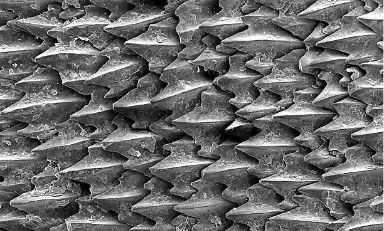
\includegraphics[scale=0.4]{7.jpg}
    \caption{鲨鱼皮表面的V字褶皱}
    \label{sy}
\end{figure}
\sub{鲨鱼皮泳衣}
鲨鱼皮泳衣的核心技术就在于模仿鲨鱼的皮肤,衣服表面排列了上百万个细小的棘齿。它还充分融合了仿生学原理:在接缝处模仿人类的肌腱,为运动员向后划水时提供动力;在布料上模仿人类的皮肤,富有弹性。Speedo最新的第四代泳衣采用了LZR Pulse面料,不仅超轻、超低阻,而且还有极佳的防水和快干性能,是全球首套以高科技熔接生产的无皱褶比赛泳衣。

但关于鲨鱼皮泳衣的效能还有不同的声音,据英国《每日邮报》报道,哈佛大学的劳德教授认为,``鲨鱼在水中前进时主要是依靠头部、背鳍和胸鳍来稳定方向,而通过尾鳍的不断摆动来提速。因此我认为鲨鱼头部和上半身皮肤表面的凸起物主要是用来引导水流通过、减少水流阻力的,而其尾部皮肤的凸起物则能够起到增强推动力的作用。'',``目前我们所认识的鲨鱼皮泳衣其实并非是通过模拟鲨鱼皮肤构造来提高穿着者在水中的移动速度的。实际上,由于鲨鱼皮泳衣特殊的材质能够紧贴皮肤,因此增加了人体体表静脉回流的速度,使得穿着者即使在肌肉疲惫时也很容易保持某个姿势,因此让人产生了提速的错觉。''
\se{什么是可再生能源?有哪些典型的可再生能源?}
根据国际能源署可再生能源工作小组,可再生能源是指“从持续不断地补充的自然过程中得到的能量来源”,它相对于不可再生能源是一种取之不尽用之不竭的能源。这里的可再生应该理解为在人类能接受的时间内就能再生,而不像石油,煤炭那样经过上亿年才能由生物转化出来。可再生能源归根结底都来自于太阳能,例如风能来自于温度梯度,潮汐能来自于引力变化。

以下是为人类使用再生能源的原因
\rk{
    \item 科技的进步让此类能源更加“好用”。
    \item 化石能源是有限的,所以其价格会日渐增涨。
    \item 某些再生能源(如风能,水力,太阳能)不会排放温室气体,如二氧化碳,因此不会增加温室效应的风险。
    \item 为了增进能源供应安全,减少对进口化石能源的依赖,并追求可持续性能源的需求。
}
\sub{典型的可再生能源}
\rk{
    \item 木材。\\柴是最早使用的典型的生物质能源,烧柴在煮食和提供热力很重要,它可让人们在寒冷的环境下仍可生存。
    \item 水能。\\磨坊就是采用水能的好例子。而水力发电更是现代的重要能源,尤其是中国、加拿大等满是河流的国家。
    \item 风能。\\人类已经使用了风力几百年了。如风车,帆船等。
    \item 太阳能。\\自古人类懂得以阳光晒干物件,并作为保存食物的方法,如制盐和晒咸鱼等。
    \item 地热能。\\人类很早以前就开始利用地热能,例如利用温泉沐浴、医疗,利用地下热水取暖、建造农作物温室、水产养殖及烘干谷物等。
    \item 海洋能。\\海洋能即是利用海洋运动过程来生产的能源,海洋能包括潮汐能、波浪能、海流能、海洋温差能和海水盐差能等,一些沿海国家的海岸线,就很适合用来作潮汐发电。
    \item 生物能。\\生物质能是指能够当做燃料或者工业原料,活着或刚死去的有机物。生物质能最常见于种植植物所制造的生质燃料,或者用来生产纤维、化学制品和热能的动物或植物。许多的植物都被用来生产生物质能,包括了芒草、柳枝稷、麻、玉米、杨属、柳树、甘蔗和沼气(甲烷)牛粪等。
}
\se{硅是地壳所含的最主要的元素之一,列举1、2种硅元素的重要应用并加以描述。}
\sub{硅用于太阳能电池板}
用单晶硅制作的电池板在受到光照射时,透过适当的能阶设计,利用光生伏打现象,便可有效的吸收太阳所发出的光,并产生电压与电流。

在P-N半导体接合处,由于有效载流子浓度不同而造成的扩散,将会产生一个由N指向P的内建电场,因此当光子被接合处的半导体吸收时,所产生的电子将会受电场作用而移动至N型半导体处,空穴则移动至P型半导体处,因此便能在两侧累积电荷,若以导线连接,则可产生电流,而太阳能电池的挑战就在于如何将产生的电子空穴对在复合之前将其搜集起来。

当前,晶体硅材料(包括多晶硅和单晶硅)是最主要的光伏材料,其市场占有率在90\%以上,而且在今后相当长的一段时期也依然是太阳能电池的主流材料。多晶硅材料的生产技术长期以来掌握在美、日、德等3个国家7个公司的10家工厂手中,形成技术封锁、市场垄断的状况。多晶硅的需求主要来自于半导体和太阳能电池。按纯度要求不同,分为电子级和太阳能级。其中,用于电子级多晶硅占55\%左右,太阳能级多晶硅占45\%,随着光伏产业的迅猛发展,太阳能电池对多晶硅需求量的增长速度高于半导体多晶硅的发展,预计到2008年太阳能多晶硅的需求量将超过电子级多晶硅。 1994年全世界太阳能电池的总产量只有69MW,而2004年就接近1200MW,在短短的10年里就增长了17倍。
\sub{氮化硅陶瓷}
氮化硅陶瓷,是一种烧结时不收缩的无机材料陶瓷。氮化硅的强度很高,尤其是热压氮化硅,是世界上最坚硬的物质之一。具有高强度、低密度、耐高温等性质。\ce{Si3N4}陶瓷是一种共价键化合物,基本结构单元为[\ce{SiN4}]四面体,硅原子位于四面体的中心,在其周围有四个氮原子,分别位于四面体的四个顶点,然后以每三个四面体共用一个原子的形式,在三维空间形成连续而又坚固的网络结构。

\ce{Si3N4}陶瓷材料作为一种优异的高温工程材料,最能发挥优势的是其在高温领域中的应用。\ce{Si3N4}今后的发展方向是:
\rk{
    \item 充分发挥和利用\ce{Si3N4}本身所具有的优异特性。
    \item 在\ce{Si3N4}粉末烧结时,开发一些新的助熔剂,研究和控制现有助熔剂的最佳成分。
    \item 改善制粉、成型和烧结工艺。
    \item 研制\ce{Si3N4}与SiC等材料的复合化,以便制取更多的高性能复合材料。
    \item \ce{Si3N4}陶瓷等在汽车发动机上的应用,为新型高温结构材料的发展开创了新局面。
}
    它极耐高温,强度一直可以维持到1200℃的高温而不下降,受热后不会熔成融体,一直到1900℃才会分解,并有惊人的耐化学腐蚀性能,能耐几乎所有的无机酸和30\%以下的烧碱溶液,也能耐很多有机酸的腐蚀;同时又是一种高性能电绝缘材料。
它极耐高温,强度一直可以维持到1200℃的高温而不下降,受热后不会熔成融体,一直到1900℃才会分解,并有惊人的耐化学腐蚀性能,能耐几乎所有的无机酸和30\%以下的烧碱溶液,也能耐很多有机酸的腐蚀;同时又是一种高性能电绝缘材料。
\se{表征材料的亲水和疏水特性的参数是什么?利用材料的超亲水和超疏水特性分别是如何实现物体的表面清洁的?}
\sub{表征材料的亲水和疏水特性的参数}
根据热力学的理论,物质会寻求存在于最低能量的状态,而关键便是个可以减少化学能的办法。水是极性物质,并因此可以在内部形成氢键,这使得它有许多独别的性质。疏水物通常是非极性的,它们无法形成氢键,所以水会对疏水物产生排斥,而使水本身可以互相形成氢键。这即是疏水作用。相对的,亲水性分子,或者说分子的亲水性部分,是指其有能力极化至能形成氢键的部位,并使其对油或其他疏水性溶液而言,更容易溶解在水里面。

\begin{figure}[htbp]
    \centering
    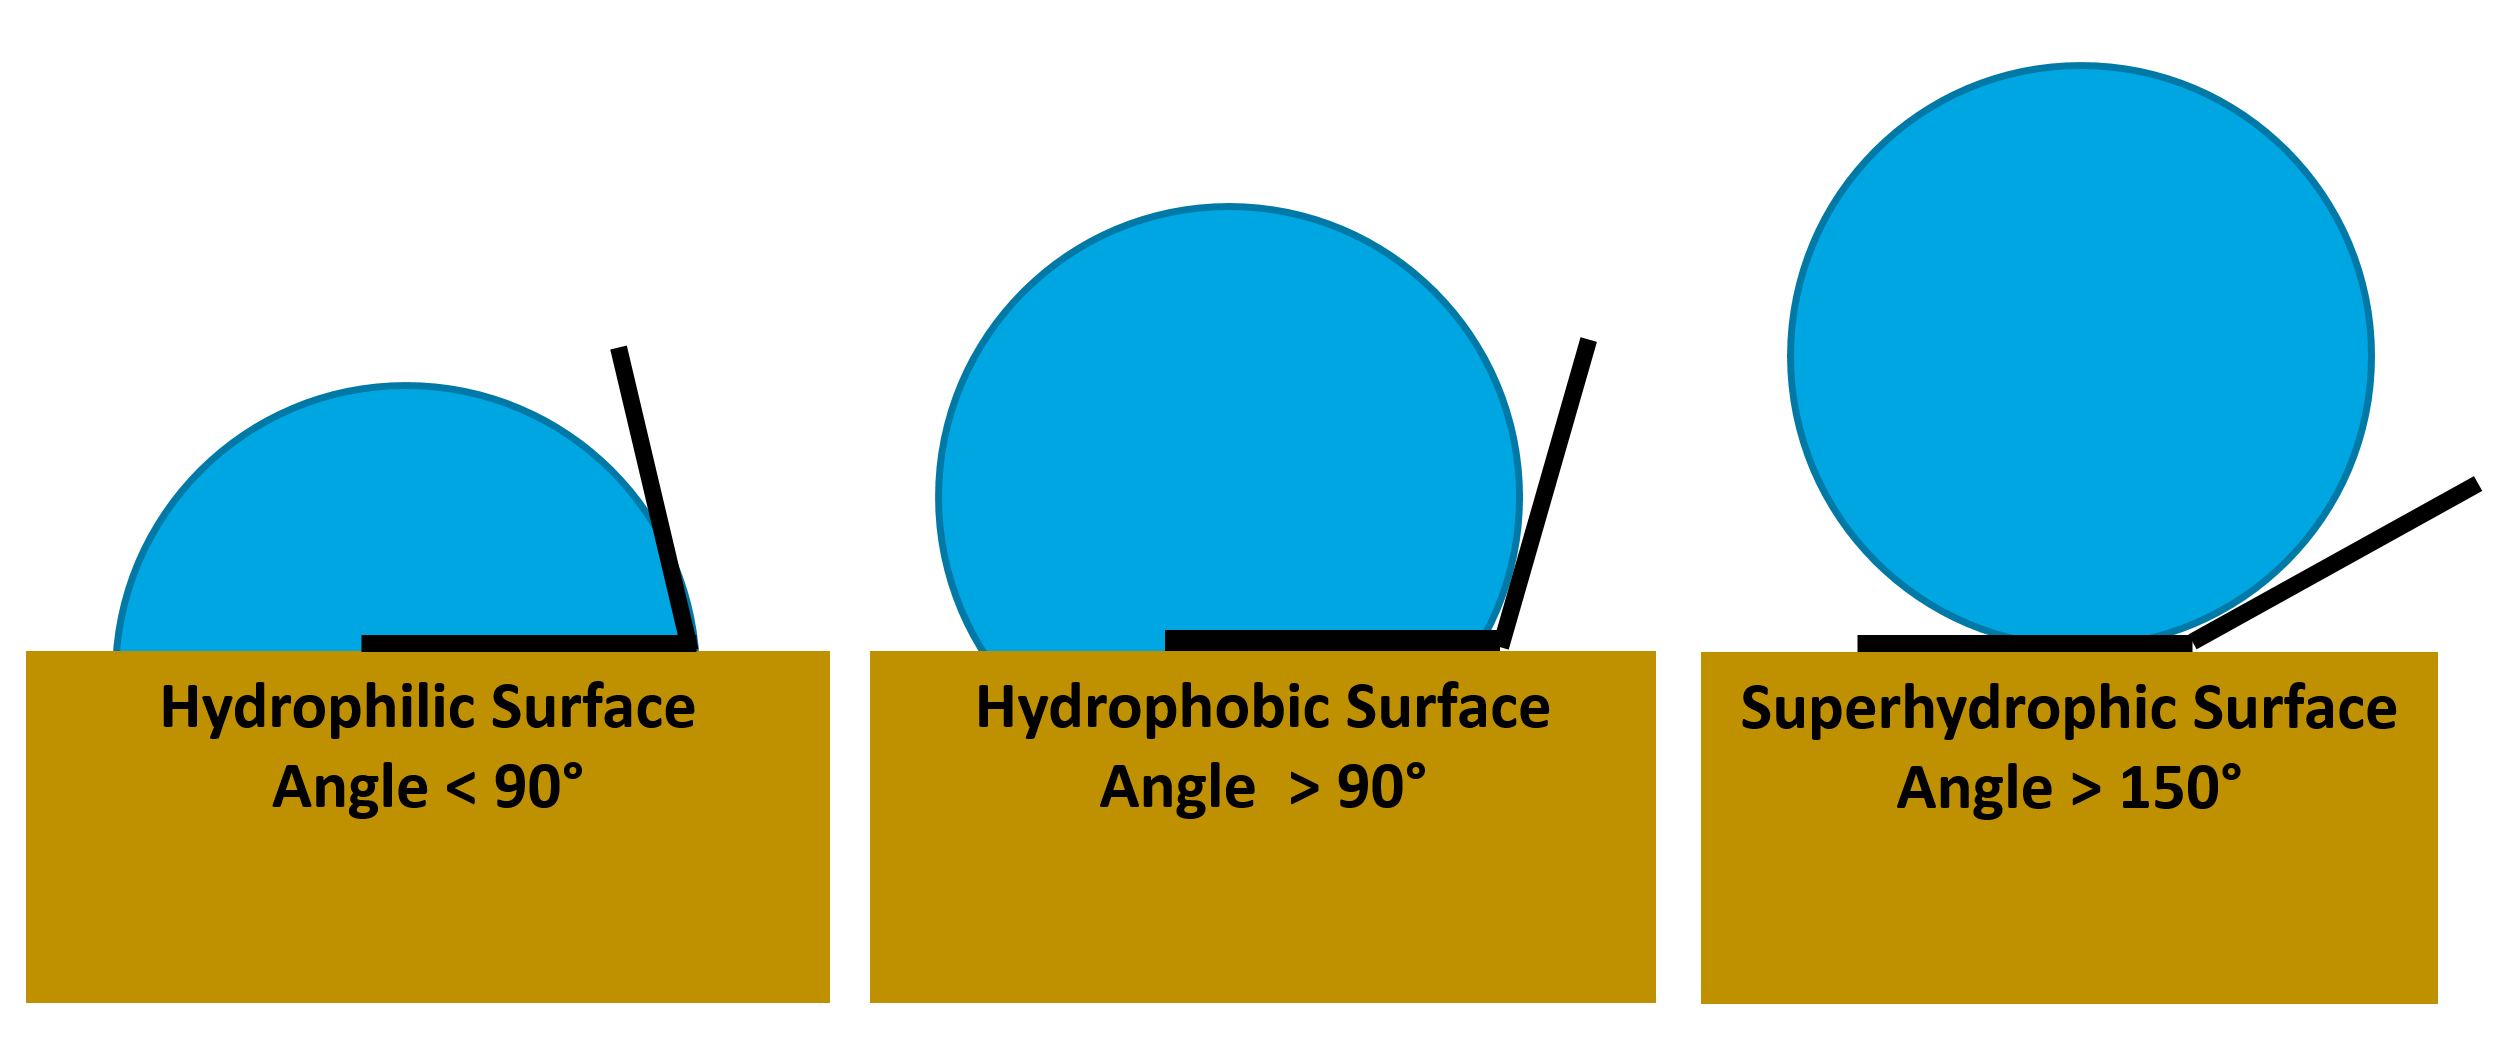
\includegraphics[scale=0.1]{9.png}
    \caption{气体环绕的固体表面的液滴,形成接触角$\t$。}
    \label{ss} 
\end{figure}
衡量材料疏水性的参数是接触角$\t$(如图 \ref{ss})。由$\t$角的大小可估计润湿程度。$\t$角越小,润湿性越好。如$\t=0$°,材料完全润湿;$\t<90$°(如玻璃、混凝土及许多矿物表面),则为亲水性的;$\t>90$°(如水滴在石蜡、沥青表面)为疏水性的;$\t=180$°时,则为完全不润湿。
\sub{超亲/疏水结构表面清洁}
超亲水和超疏水自清洁表面都是利用了材料表面的特殊浸润性。\\
一方面,水在超亲水表面上会自发铺展成面积很大而厚度很薄的水膜,阻碍了油脂和灰尘微粒等污染物与表面的直接接触 ;而完全铺展的水膜又会很快蒸发 ,带走其表面附着的杂质,实现自清洁功能。自然界中,蜗牛壳就属于这种情况。工业上,超亲水表面目前多以防雾自清洁涂层或薄膜的形式应用在一些比较特殊的环境中,例如骑车后视镜,齿科或体内专用的窥镜,以及一些比较高级眼镜片等等。\\
另一方面,水在超疏水会自发形成聚拢的水滴,当水滴在倾斜表面上滚动时,会自发带走表面附着的一些灰尘颗粒,实现自清洁功能。自然界中,除了之前提到的荷叶之外,一些蝴蝶的翅膀也具有类似功能。工业界中,则主要应用于大型建筑的玻璃外墙等难以清洁的表面等。
\se{气垫层是自然界中生物和动物形成超疏水的重要原因,请进行具体描述和说明。}
接触角可通过式 \ref{shi}计算。
\begin{equation}
\gamma_{S G}=\gamma_{S L}+\gamma_{L G} \cos \theta \label{shi}
\end{equation}
其中
$$ 
\begin{aligned} 
    \gamma_{S G} &=\text{固体和气体之间的表面张力}\\ 
    \gamma_{S L} &=\text{固体和液体之间的表面张力}\\ 
    \gamma_{L G} &=\text{液体和气体之间的表面张力}
\end{aligned}
 $$
 \begin{figure}[htbp]
    \centering
    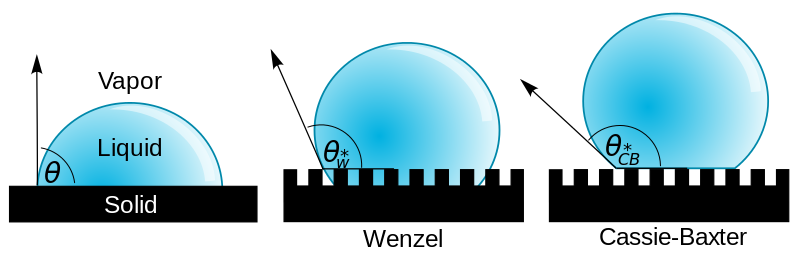
\includegraphics[scale=0.4]{8.png}
    \caption{气体环绕的固体表面的液滴,形成接触角$\t$。如果液体与固体表面微结构的凹凸面直接接触,则此液滴处于Wenzel状态;而如果液体只是与微结构的凸面接触,则此液滴处于Cassie-Baxter状态。}
     
\end{figure}
 当液体直接接触微结构化的光滑表面时 (Wenzel状态),$\t$角会转变为$\theta _{W}*$
 $$ 
\cos \theta_{W*}=r \cos \theta
 $$
 其中,$r$为实际面积与投影面积的比率。\\
 如果液体悬浮在粗糙的微结构表面,$\t$角将会变为$\theta _{{CB}}*$
\begin{equation}
\cos \theta_{C B} *=\varphi(\cos \theta+1)-1 \label{cb}
\end{equation}
 其中,$\vp$为固体与液体接触面积的比例。

Cassie-Baxter模型即是一种气垫模型。模型指出,液体在粗糙的表面的接触是一种复合接触。这个模型可以很好地解释Wenzel模型不能解释的超疏水表面的性能表现。根据式 \ref{cb},当接触面积比例变小,即$\vp\rightarrow 0$时,$\cos \theta_{C B} *\rightarrow -1$,接触角变得相当大。因此气垫层的存在可以让超疏水性质更好。
\se{柔性可穿戴电子产品有哪些相关技术?列举一种实现柔性电子产品的技术进行描述。}
\sub{柔性可穿戴电子传感器机械力信号转换}
机械运动的传感器能有效地将外部刺激转化为电信号,是柔性可穿戴电子传感器监测身体健康状况的关键技术。柔性可穿戴电子传感器的信号转换机制主要分为压阻、电容和压电三大部分(见图 \ref{rx})。
\begin{figure}[htbp]
    \centering
    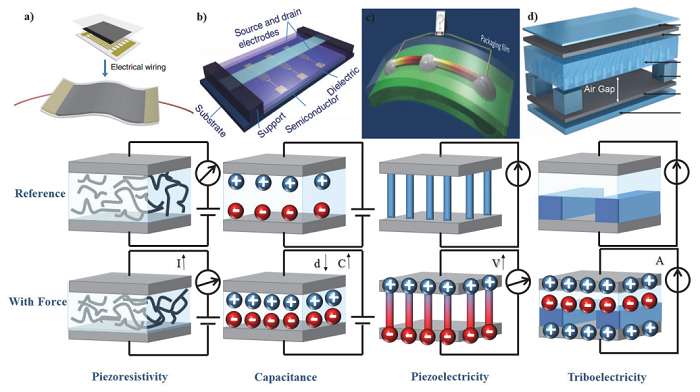
\includegraphics[scale=0.4]{10.png}
    \caption{柔性可穿戴电子传感器四种信号传导机制和器件的示意图}
    \label{rx} 
\end{figure}
\sub{柔性可穿戴电子的常用材料}
\rk{
    \item 柔性基底\\
    为了满足柔性电子器件轻薄、透明、柔性和拉伸性好、绝缘耐腐蚀等性质的要求,方便易得、化学性质稳定、透明和热稳定性好聚二甲基硅氧烷(PDMS)成为了人们的首选,尤其在紫外光下粘附区和非粘附区分明的特性使其表面可以很容易的粘附电子材料。目前,通常有两种策略来实现可穿戴传感器的拉伸性(见图 \ref{rx2})。第一种方法是在柔性基底上直接键合低杨氏模量的薄导电材料。第二种方法是使用本身可拉伸的导体组装器件。通常是由导电物质混合到弹性基体中制备。
    \begin{figure}[htbp]
        \centering
        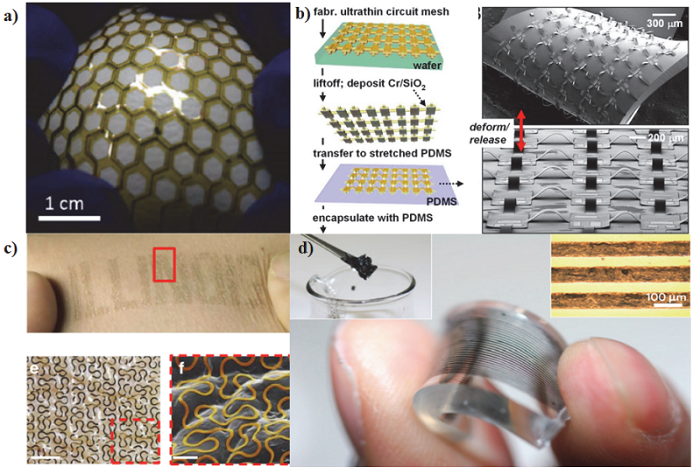
\includegraphics[scale=0.3]{11.png}
        \caption{实现可拉伸性的不同策略}
        \label{rx2} 
    \end{figure}
    \item 金属材料\\
    金属材料一般为金银铜等导体材料,主要用于电极和导线。对于现代印刷工艺而言,导电材料多选用导电纳米油墨,包括纳米颗粒和纳米线等。金属的纳米粒子除了具有良好的导电性外,还可以烧结成薄膜或导线。
    \item 无机半导体材料\\
    \begin{figure}[htbp]
        \centering
        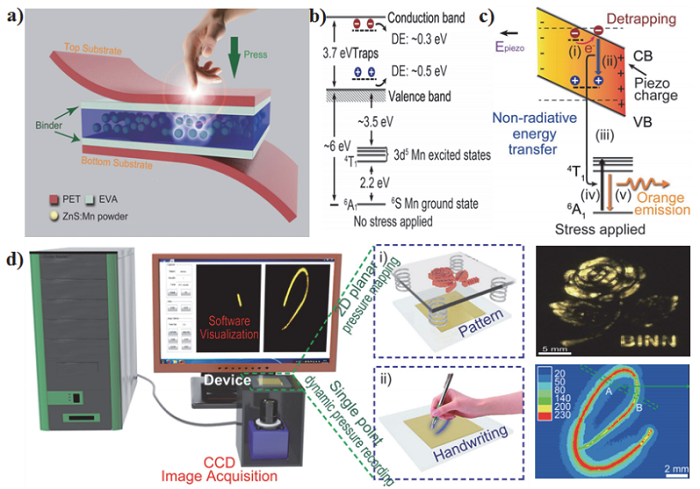
\includegraphics[scale=0.3]{12.png}
        \caption{基于力致发光的压力扫描}
        \label{rx3} 
    \end{figure}
    以ZnO和ZnS为代表的无机半导体材料由于其出色的压电特性, 在可穿戴柔性电子传感器领域显示出了广阔的应用前景。一种基于直接将机械能转换为光学信号的柔性压力传感器被开发出来(见图 \ref{rx3})。这种矩阵利用了ZnS:Mn颗粒的力致发光性质。力致发光的核心是压电效应引发的光子发射。压电ZnS的电子能带在压力作用下产生压伏效应而产生倾斜, 这样可以促进\ce{Mn^{2+}}的激发,接下来的去激发过程发射出黄光 (580 nm左右)。

    \item 有机材料\\
    典型的场效应晶体管是由源极、漏极、栅极、介电层和半导体层五部分构成。根据多数载流子的类型可以分为p型(空穴)场效应晶体管和 n 型(电子)场效应晶体管。传统上用于场效应晶体管研究p型聚合物材料主要是噻吩类聚合物,其中最为成功的例子便是聚(3-己基噻吩)(P3HT)体系。萘四酰亚二胺(NDI)和苝四酰亚二胺(PDI)显示了良好的 n型场效应性能,是研究最为广泛的n型半导体材料,被广泛应用于小分子n型场效应晶体管当中。

    \begin{figure}[htbp]
        \centering
        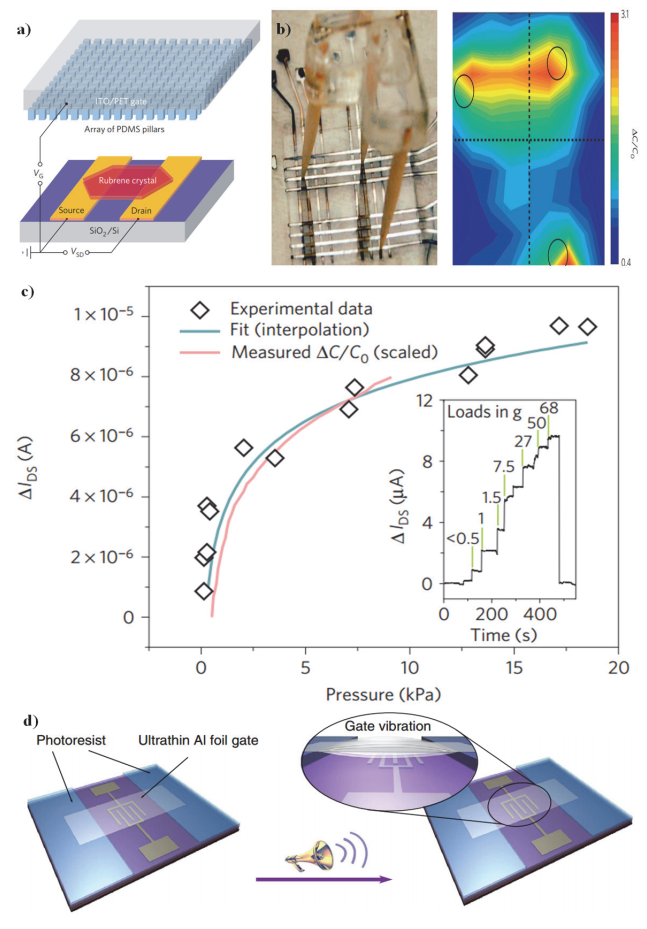
\includegraphics[scale=0.3]{13.png}
        \caption{基于栅介电层几何设计的高灵敏的矩阵传感器}
        \label{rx4} 
    \end{figure}
    为了满足更多的应用,人们亟需发展一种检测压力范围广,响应速度快的矩阵策略。鲍哲楠等在硅片上集成了一种新型高压敏感的有机晶体管,其具有微结构的可压缩栅电介质(见图 \ref{rx4})。相比于无结构或其他微结构的膜,具有锥状结构的PDMS层电容式传感器极大地提高了压力敏感性。原因是 PDMS 层和有机半导体间空隙的提高使得介电常数降低。在此基础上, 进一步在塑料基底上发展了柔性的压敏矩阵。 这种基于微结构橡胶的矩阵具有反应迅速和高压敏感性的特点,其可以精确的扫描静态压力分布和监测健康。

    \item 碳材料\\
    柔性可穿戴电子传感器常用的碳材料有碳纳米管和石墨烯等。碳纳米管具有结晶度高、导电性好、比表面积大、微孔大小可通过合成工艺加以控制,比表面利用率可达 100\%的特点。 石墨烯具有轻薄透明,导电导热性好等特点。
}
\sub{柔性电子传感器的印刷制造}
与传统自上而下的光刻技术相比, 印刷电子技术拥有弯曲与拉伸性好、可以在柔性基底大规模制备、加工设备简单、成本低和污染小等优点。这种新型图案化技术可以简便地进行纳米粒子微、纳米尺度图案的精确组装, 可以通过“印刷”方式大面积制备纳米粒子组装的精细图案和功能器件,乃至实现单个纳米粒子的组装与图案化;通过喷墨打印技术构筑微米尺度的电极图案作为“模板”,控制纳米材料的组装过程成功制备了最高精度可达30 nm的图案,并实现了柔性电路的应用。
\begin{figure}[htbp]
    \centering
    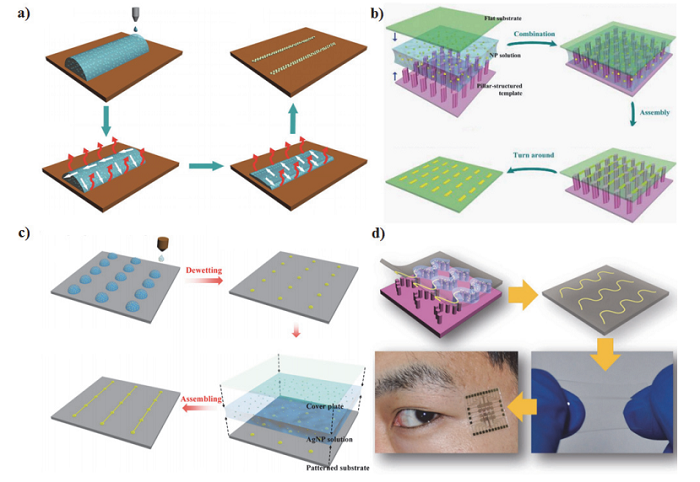
\includegraphics[scale=0.4]{14.png}
    \caption{印刷电子的精细图案化控制}
\end{figure}
\sub{柔性锂离子电池技术}
表 \ref{tu}是这是几类可折叠电子设备的曲率(点鼠标),可以看到,可折叠电子设备对材料弯折性能的要求相当高,作为对照,日常生活中可塑性比较高的铝仅能在0.6\%的曲率下多次弯曲不受损,传统的电池将多层组件堆叠在一起,轻微的弯曲就会导致脱层和活性材料的损坏。因此要生产用于这样设备的电池必然要有完全不同的结构。于是柔性锂离子电池 (LIBs)技术开始受到关注。

\begin{figure}[htbp]
    \centering
    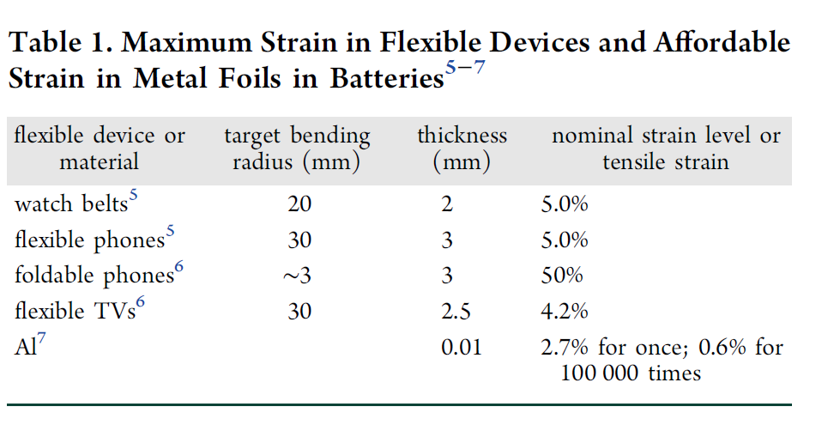
\includegraphics[scale=0.7]{15.png}
    \caption{几类可折叠电子设备的曲率}
    \label{tu}
\end{figure}

表 \ref{tu2}是目前上已实现商业化的各种柔性电池及其属性,最左边一列是它们的设计原理,这几种设计各有优缺点。未来,新型材料、器件结构和制造技术的发展将进一步提高柔性LIBs的性能,特别是实现更小的弯曲半径、更高的能量密度和更大的弯曲周期。

\begin{figure}[htbp]
    \centering
    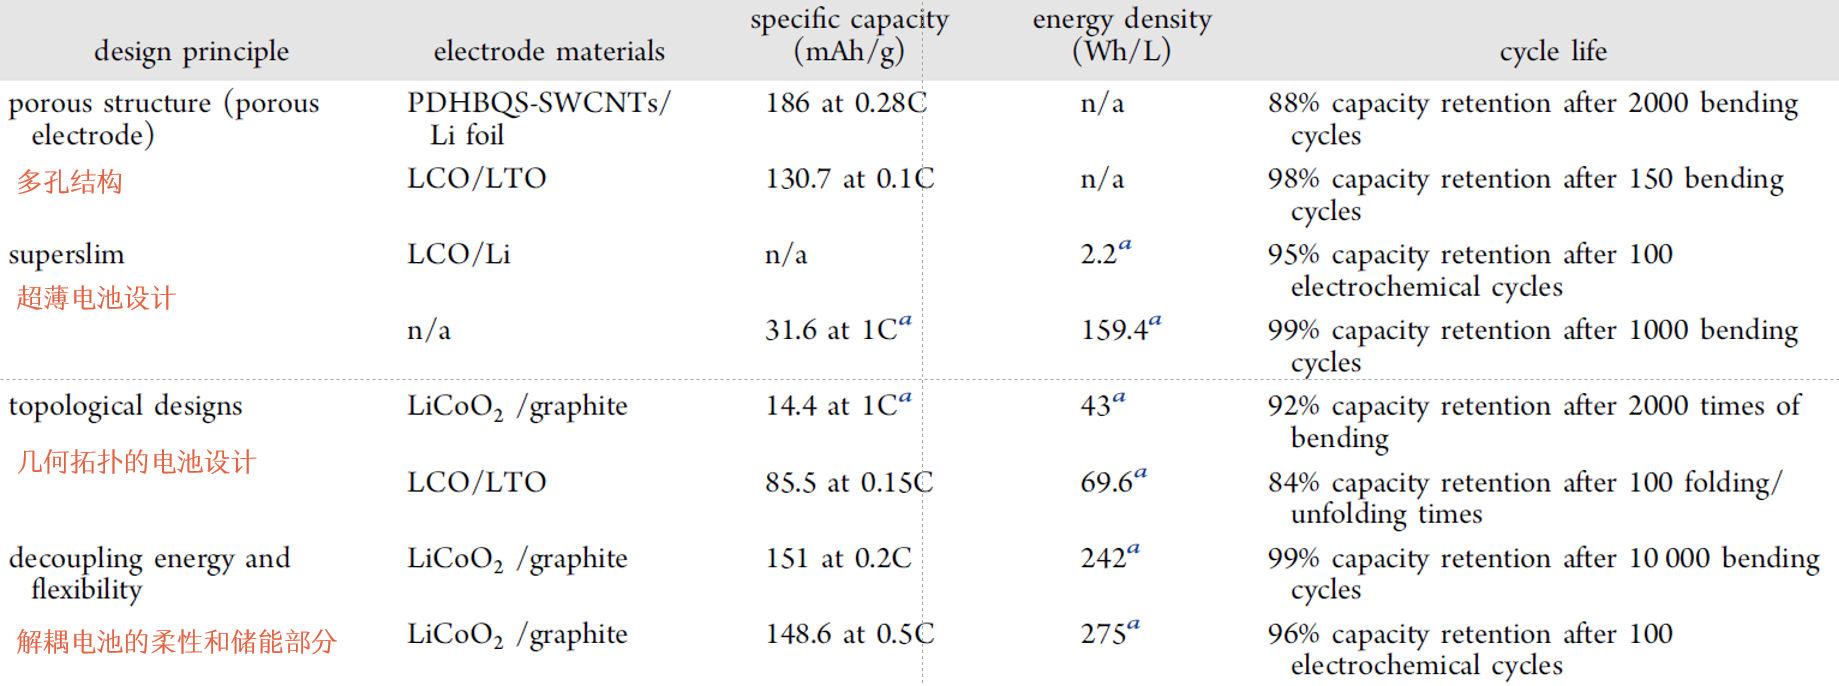
\includegraphics[scale=0.3]{1_4.png}
    \caption{各类柔性电池}
    \label{tu2}
\end{figure}

图 \ref{ldc1}是RGO在高温下具有机械柔性,右图为磷酸铁锂的SEM图像。实验人员吧复合阴极涂在RGO电流收集器上,表现出良好的接触性。我们刚才说了一块良好的电池要有稳定的电流输出,也就是在弯曲的时候阻抗变化要小。经验上,这种阻抗主要来自于界面接触不良,图中这样良好接触的封装有助于阻抗的降低。

\begin{figure}[htbp]
    \centering
    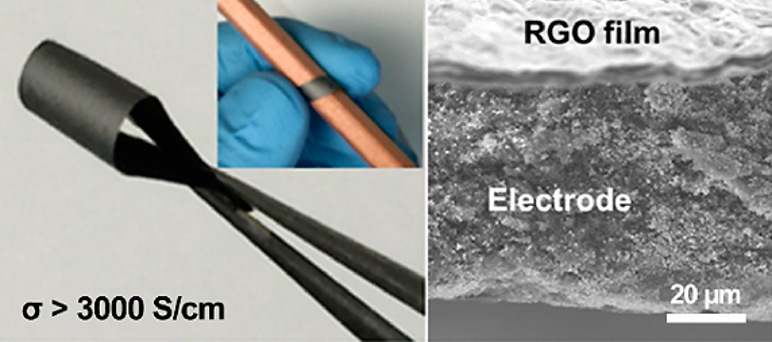
\includegraphics[scale=0.5]{16.png}
    \caption{Liangbing Hu等人报道了一种氧化石墨烯导电多孔薄膜 (RGO),它具有的导电率高达3112 S/cm。用此薄膜作为集流体装配的柔性锂电池,在高充放电倍率(5C)循环100次后,并未发现容量的明显衰减。}
    \label{ldc1}
\end{figure}

图 \ref{ldc2}显示了这个正极材料良好的柔韧性。右边这个是电池容量与循环数之比,绿色的这个插图显示了这个聚合物的弯曲和平面两种状态。这种设计把碳纳米管和与这个聚合物化合在一起,可以有更大的电容量和出色的放电速率。单臂碳纳米管兼具集电性和导电性,可以把机械稳定性提高,经过2000次弯曲后仍能保持88\%的容量。

\begin{figure}[htbp]
    \centering
    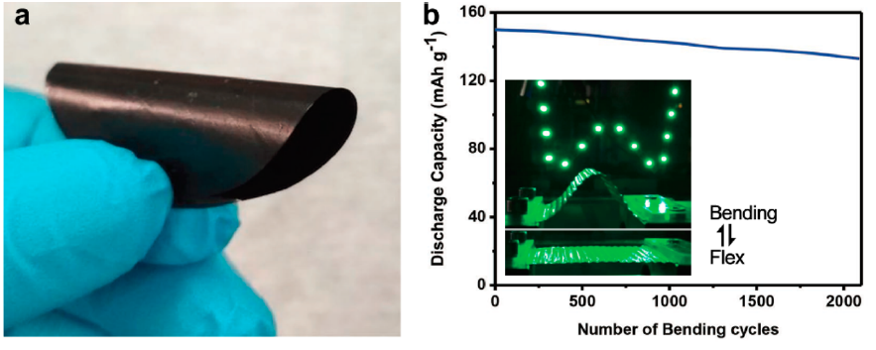
\includegraphics[scale=0.5]{17.png}
    \caption{一种单壁碳纳米管与聚合物(2,5-二羟基-1,1-苯并醌基硫化物)复合的正极材料被用于装配柔性锂电池。该电池在低电流下(50 mA/g)展现出了182 mAh/g 的放电比容量,在超大电流下(5000 mA/g)放电时,仍可达到75 mAh/g 的比容量。}
    \label{ldc2}
\end{figure}

图 \ref{ldc3}展示了一种以细菌纤维素为模板的电解质设计,左边是以细菌纤维素为模板的电解质的示意图,右边显示了这种电解质的柔软性。

\begin{figure}[htbp]
    \centering
    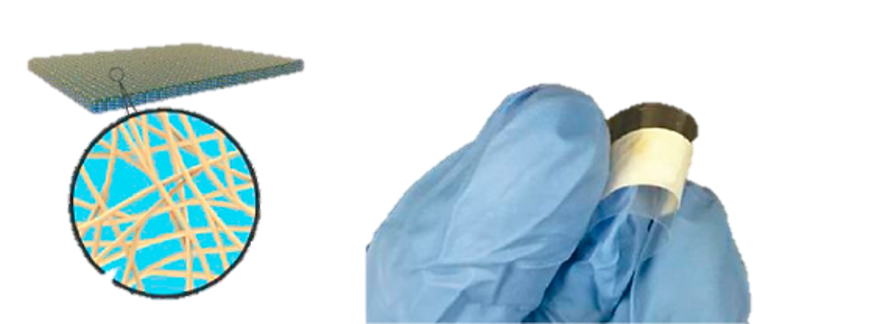
\includegraphics[scale=0.5]{18.png}
    \caption{一种单壁碳纳米管与聚合物(2,5-二羟基-1,1-苯并醌基硫化物)复合的正极材料被用于装配柔性锂电池。该电池在低电流下(50 mA/g)展现出了182 mAh/g 的放电比容量,在超大电流下(5000 mA/g)放电时,仍可达到75 mAh/g 的比容量。}
    \label{ldc3}
\end{figure}

\se{什么是3D打印技术,举例说明3D打印技术的应用。}
\sub{3D打印技术}
“3D打印”这个词的原意是指将材料有序沉积到粉末层喷墨打印头的过程。现扩大到指任何打印三维物体的过程。3D打印的内容可以来源于三维模型或其他电子数据,其打印出的三维物体可以拥有任何形状和几何特征。3D打印机属于工业机器人的一种。

3D打印分为3步,建模,修正,打印。

3D打印模型可以使用计算机辅助设计软件包或三维扫描仪生成。手动搜集制作3D图像所需的几何数据过程同雕塑等造型艺术类似。通过3D扫描,可以生成关于真实物体的形状、外表等的电子数据并进行分析。以3D扫描得到的数据为基础,就可以生成被扫描物体的三维计算机模型。

模型建立好后,打印3D模型前需要先进行“流形错误”检查,这一步通常称为“修正”。对于采用3D扫描获得的模型来说,STL文件“修正”尤其重要,因为这样的模型通常会有大量流形错误。

最后,3D打印机从不同的横截面将液体,粉末,纸张或板材等材料一层层组合在一起。这些层次与计算机辅助设计模型中的虚拟层次都是相对应的。这些真实的材料层或人工或自动地拼接起来形成3D打印成品。3D打印技术的主要优势在于,它几乎可以打印所有形状的物品。
\sub{3D打印技术的应用}
今年4月,一篇发表在Nature Communications上的文章找到了使用透明头骨植入物在老鼠大脑打开一个窗口的方法。这种方法被称之为“See-Shell”。研究人员对鼠标的头骨进行数字扫描,并使用数据使用3D打印机创建匹配的透明片。然后用See-Shell手术替换头骨。

\begin{figure}[htbp]
    \centering
    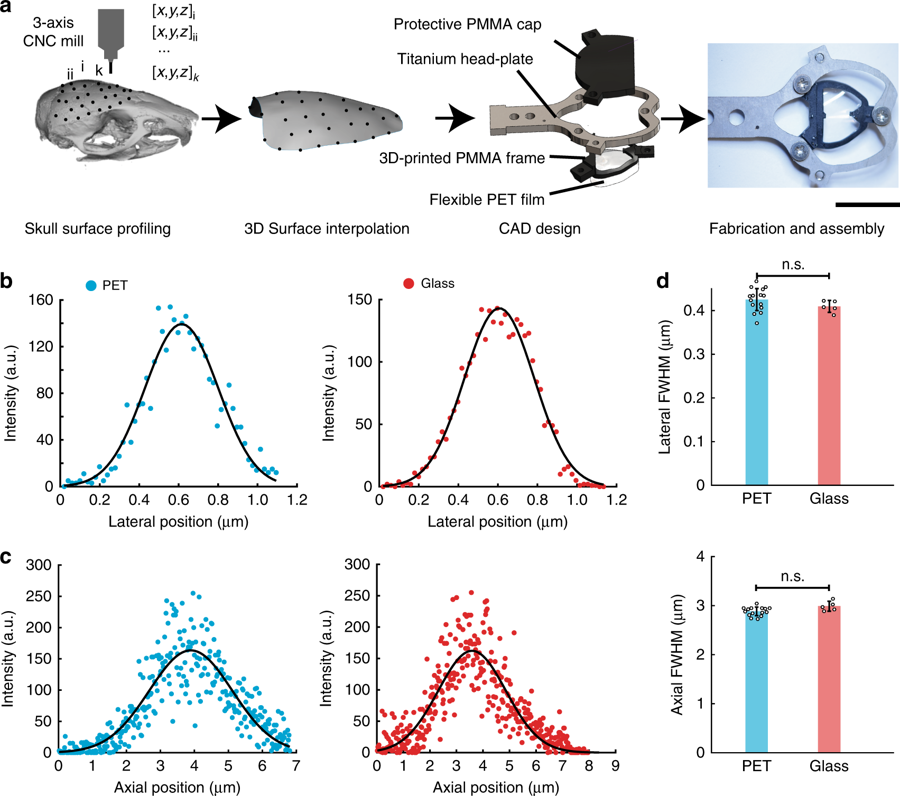
\includegraphics[scale=0.35]{19.png}
    \caption{这个头骨表面轮廓是用来插值一个三维表面。以三维表面为模板,设计形态一致的透明种植体(see-shell),该透明种植体由3D打印聚甲基丙烯酸甲酯(PMMA)框架构成,框架上粘接一层薄的、光学透明的、柔性的聚对苯二甲酸乙二醇酯(PET)薄膜。固定在框架上的钛头板提供固定头部的机械支撑,3d打印的帽子保护植入物和下方的脑组织。右图显示的是一个完全制作和组装的See-Shell。标尺表示1厘米。}
\end{figure}

See-Shell可以帮助科学家研究各种人类大脑状况,如脑震荡,阿尔茨海默氏症和帕金森病等退行性疾病。神经科学家Timothy Ebner说:“这些是在我们人类身上无法做到的研究,但它们对我们对大脑如何运作非常重要,因此我们可以改善对脑部受伤或疾病患者的治疗方法。”
\se{列举一种材料回收利用的技术。}
\sub{复合软包装材料回收利用研究进展}
随着包装技术的发展,复合软包装由于其具有质轻、柔软、废料少、占有空间少、成本低以及成本有效性高(单位重量包装的体积和重量)等优点,近几年来,它在世界范围内得到广泛重视和迅速发展。但与此同时,复合软合包装废弃物的数量也与日俱增,它一方面来源于复合生产过程中的废膜、废料及边角料,据统计,一个l年生产50吨的复合薄膜生产厂,每年约有10吨废料产生,另一方面来源于使用完毕后形成的复合包装废弃物。
\sub{纸塑复合包装回收利用}
据分析估测,我国每年使用纸塑复合材料达10万吨以上,而且还以惊人的速度增长,将废旧纸塑材料变废为宝,实现了资源循环综合利用,保护环境,具有巨大的经济效益和社会效益。目前国内出现了多种回收处理方法,如以废弃的纸塑复合材料为原料,用有机溶剂溶解分离出纸单体后,进行打浆造纸工序,原料在有有机溶剂的溶解槽内,经加热、搅拌,溶解纸塑复合材料的塑料层,分离纸单体和其他单体层,干燥后,分选出纸片打浆造纸;将纸塑复合材料的纸面平放置加热板上,通过加热板加热,其加热温度在150℃-280℃之间,加热时间20-50秒之间,通过加热使纸塑的塑胶收缩变形,从而与纸面分离。
\sub{纸铝塑复合包装材料回收利用}
纸铝塑复合包装材料利用纸张的挺度、铝的阻隔性及塑料的热封性和热粘性,在包装中应用十分广泛。这种包装结构在瑞典利乐公司生产的利乐包中应用最多,目前就利乐无菌包装废弃物再回收利用的技术有: \rk{
    \item 水力再生浆技术\\
    将利乐包中的纸浆分离出来,生产再生纸; 而将利乐包中的塑料和铝成分挤压成粒,成为生产塑料和铝制品很好的原料。
    \item 塑木技术\\
    利乐包本身包含优质的纸质纤维和塑料,把它们碾碎挤压,生产塑木产品,正是物尽其用,成本低廉。用废弃利乐包生产的室内家具、室外园艺设施、工业托盘等等,都广受消费者的欢迎和好评。
    \item 彩乐板技术\\
    将废弃利乐包直接粉碎、热压处理,制成彩乐板,它是以复合包装物中的塑料为主要胶粘剂,纸,铝箔及其他纤维为增强材料,在一定的添加剂作用及高温高压下,经加压平整定型等工艺压制而成。彩乐板可以制成多种产品,尤其是果皮箱,既美观、耐用又成本低廉。
}

\begin{figure}[htbp]
    \centering
    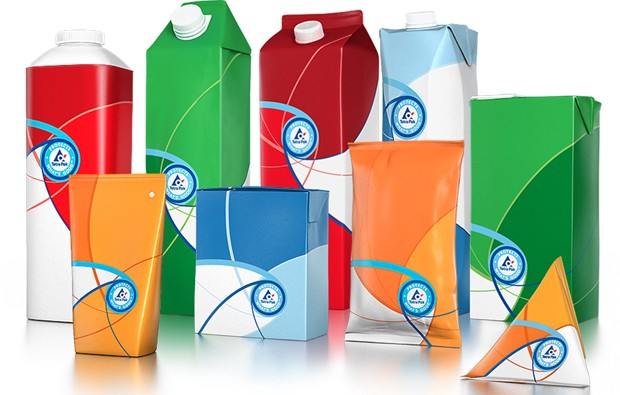
\includegraphics[scale=0.35]{20.jpeg}
    \caption{各种利乐包}
\end{figure}

\se{列举2种由自然界物质引发的新材料技术思维并进行具体描述(不少于1500字)。}
\sub{分子强力胶}
分子强力胶是2013年牛津大学生物化学系的马克·豪沃思和他的研究组发现的一种从化浓性链球菌侵入细胞后所放出的蛋白结合而成的胶。其超强黏合力无与伦比,能将蛋白质分子黏在一起。这种胶可以用来“抓住”蛋白质,或者把蛋白质黏在物体表面,甚至用它来组装蛋白质和酶,黏合各种纳米结构。无论是在生物技术还是纳米技术领域,都是一件有用的工具。

分子强力胶的灵感来自于许多人咽喉都携带有的化脓链球菌。这种蛋白质非常特殊,它能自发地与自己发生反应,形成一把锁扣。一般来说,蛋白质的三级结构来自于疏水残基的包埋和少数的氢键等,这些都是一些分子间残留的电性作用,但化脓链球菌中的FbaB蛋白的三维结构也是由共价键形成,这种强力化学键能在一瞬间就将氨基酸链连接成极牢固的环。

研究人员先沿着超级共价键把蛋白质拆解开,把其中较大的一半昵称为“捕谍器”(SpyCatcher),较小一半叫“谍标签”(SpyTag)。然后再让它们碰在一起,结果能再次结合形成强力共价键。这两部分,也包括跟它们黏附在一起的任何东西,也都牢牢地钉在一起。

研究人员还用原子力显微镜测试了要多大力量才能让“谍标签”脱离“捕谍器”的掌握。他们向外拉两端时,直到拉它们的工具先破裂了,这两部分仍然牢牢黏在一起;即使在洗涤剂中煮沸了,它们也没有分开。

目前已知分子强力胶有主要两个方面:\rk{
    \item 由于这种胶可与其它蛋白锁在一起,当体内癌细胞在血液中分裂时,利用分子强力胶在血液中捕获癌细胞;这可用作癌症的诊断手段;
    \item 这种分子强力胶可粘结金属,塑料及其种类物质,解决了原有各种漆都与金属粘附不强的问题,先在金属表面涂分子强力胶,后再涂其它种类漆;金属就能永久保护。
}

分子强力胶的研制大致遵循一个``从自然中发现某种不平凡的现象\ce{->}设计实验找寻现象背后的原因\ce{->}找寻潜在的应用方向\ce{->}人为重现这种现象''的路径。这是一种能高效地从身边事物提出问题,并通过一系列方法提高人类发展水平的信念体系。

在分子强力胶的发现过程中,研究人员首先提出了``为什么链球菌的蛋白质结构能黏在其他蛋白质的表面''这个问题,这个问题抽象出来就是``什么结构能产生很强的粘附力?''。其潜在的应用价值在这里就已经明晰了。

接着,研究人员通过亲自实验或是翻阅文献的方法得到了答案,是蛋白的一个特殊结构使其易于和其他氨基酸形成共价键。下一步,便是分离出这种结构,即文中的“捕谍器”和“谍标签”,发现分离后这种粘附性不会丢失。于是,研究人员模仿这种结构,设计出了同样具有超强粘附力的胶。
\sub{防水防雾防眩光的三防玻璃}
Zebra Plants是一种外表平平的植物,但它的叶片却有着不平凡的一面,这种植物的叶片不会粘上水珠,具有很好的防水性,科学家通过显微镜观察发现防水性的来源是叶片表面很多圆锥状的微结构。

\begin{figure}[htbp]
    \centering
    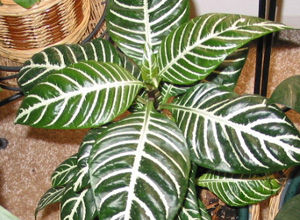
\includegraphics[scale=0.5]{21.jpg}
    \caption{斑叶肖竹芋(Zebra Plants)}
\end{figure}

在此启发之下,科学家利用半导体工业界的镀层蚀刻技术在玻璃表面“长出”了一层圆锥微结构阵列。大致过程如下:首先在玻璃表面镀上多层光敏材料(photoresistance material),其次通过控制激光刻蚀的深度和位置,用类似雕刻的手段逐渐在光敏材料上刻出一个个圆柱体的形状。精确控制圆锥的大小、锥面角度等几何参数可以改变玻璃表面的粘滞力以及折射系数等物理量,可以通过理论建模计算优化出所需要的圆锥使得表面同时具有疏水性和防眩光性(沿圆锥轴向折射率梯度变化可以有效去除全反射)。

图 \ref{sfbl}从左到右表明了圆锥体阵列的大小形貌以及演示了防水、防雾、防眩光的对比效果: 

\begin{figure}[htbp]
    \centering
    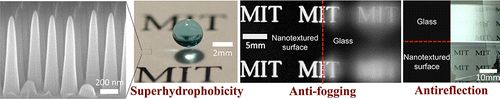
\includegraphics[scale=0.5]{22.jpg}
    \caption{圆锥体阵列的大小形貌以及演示了防水、防雾、防眩光的对比效果}
    \label{sfbl}
\end{figure}

借由这三大使用的功能,其前途不可限量,首先离我们最近的就是电子产品的显示屏,这个玻璃在广域波段上可以达到98\%的透光率,如果在我们的手机或者平板表面上放置这样的一层玻璃,那么在平时使用中可以省去不小的麻烦。其次就是在太阳能电池领域,众所周知太阳能电池上的灰尘和脏东西会减少其对光的捕获能力从而降低其效率,如果有这样的一种自清洁玻璃作为面板材料,可以保证长时间的高效率工作。

对照两种从自然界获得灵感的新材料的发明过程我们可以发现,他们几乎都遵循了相同的路线,先找到一种可能具有探究价值的现象,探究现象背后的结构,用工业的方法重现这种结构,并用以解决实际的问题。这两种发现有一个重要的特点,即在发现问题时就有了对其潜在应用的猜想。研究人员是先立足于链球菌蛋白高强度的粘附力可能可以用于制造一种强力胶再进行整个实验探究过程,先立足于植物叶片具有较好的防水性再去追问为什么。生活中大大小小的难以理解的,不平凡的生物现象处处皆是,但最具有价值的,还得是那些能够发展应用的现象。因此一双能甄别现象背后潜在的应用价值的眼睛尤为重要,某种程度上来说,一个课题选题正确的时候,就已经完成了一半。

但是,并不是短期找不到工业应用的发展方向就是无用或者错误的方向,第一,在真正弄清楚一个问题前,谁也不知道它背后隐藏了多少秘密,一个现象或者设计有没有价值在未被完全理解透之前是没有人能确定的。第二,风险与收益成正比。一个短期内无法在工业界应用的课题通常一旦问题被解决,就会给人类带来巨大的进步。这类研究通常意味着更高的风险,一旦开展研究就意味着长时间人力物力的巨大投入,而这段时间可能一直没有回报。因此我个人认为,像这类短期没有回报的,更像是对未来探索性的研究方向应该由大型企业,研究所背负起来。
\se{对本材料通识课的体会、意见和建议。}
作为一个通识类课程,同学们能够接受知识的来源几乎全部来自于上课,以及这张答卷。因此老师上课的质量的确决定了同学们能够吸收多少知识,基于这半个学期的学习,我谈一谈个人对这门课的看法。

首先,老师的确是像课程介绍那样,是面对各年级各专业的同学的,没有像我在选课时担心的那样因为课程名字里有``材料''两个字便上成了一节材料专业课。课程内容立足于``生活'',主要围绕生活中常见或者人们会感兴趣的内容,没有拘泥于一些生涩难懂的专业知识,也几次提醒同学们演讲时不需要有具体的公式等其他专业同学难以理解的内容,我认为老师是有注意保持专业和通识之间的平衡的,让同学们感受到了材料在生活中的各方各面不为人知的应用。我也的确认为这方面是这堂课令人满意的一方面。

兴趣是最好的老师,就我而言,我是物理专业的学生,尚且算是和材料比较有关,但是除了新闻推送外,平常也几乎不会主动关注材料在各方面的进展。其实大多数人对各种新材料没有概念并不是没有兴趣,而只是没有产生要去主动了解的想法。我觉得学完这节课后最大的收获还并不是课堂本身学到的内容,而是对整个新材料的行业有了一个大致的认识。以后在看到一些材料相关的新闻就会产生一种``这个东西我之前学到过''的想法,会产生一种像是看到了老朋友的感觉,于是就可能会进一步地去了解这种新材料。同时在生活中我们在看到用到各种材料时,也会时不时想起其背后各种设计的影子。这种耳濡目染的影响会反过来产生``材料的科学在生活中处处皆是''的感受。这种在课外的影响我认为才是这门课真正的魅力所在。

我也希望现在这种老师授课+同学演讲的方式继续下去。这门课的上课时间毕竟比较长,虽然老师已经尽力让授课有趣,但始终听着一个声音还是会产生一定的疲劳感,同学们每个人都各有各的讲课风格,可以给课程增加一些变化。从另一方面来看,提供了一个任务也可以促进上课效率的提高,有了这个任务之后,同学们就会或多或少地去更认真地听课看有没有能加入到自己PPT里的内容。

同时,对这种讲课方式我觉得尚有一些改进的空间。这种上课方式一个比较明显的问题就是课程会严重超时,因为大多数同学的讲课时间都超过了本来要求的时间。而下课后许多同学还有其他安排也会被耽误。例如我每天晚上九点半需要到实验室,我的队友也会这个时候等着我过去,本来9点15下课恰好可以到实验室,但如果一直不下课就会迟到,这堂课上和我一样要九点半到实验室的同学不仅有我一人,他们也只能选择提前离开或者迟到。如果老师也觉得这是一个需要解决的问题的话,我提供几种个人觉得比较可行的解决方法,希望能有所帮助:
\rk{
    \item 预估同学们讲课需要花费的时间,提前开始让同学讲课。如果大家讲的比较快或者是有的同学没有讲,提前结束了,那么老师也可以进行一些总结或者专门留一些可以在这段时间讲的内容。如果大家讲的比较慢,也不会拖得太久。当然,这个办法的缺点就是上课的时间会被压缩。
    \item 在学期开始时缩短告知的讲课时间,这样也可以更快结束,缺点是本来的时间已经不多,如果再次缩短可能让上课的内容浅尝辄止,也更难评估学生的讲课质量。
    \item 像其他一些课程一样,规定的时间到后提醒学生,同时允许学生有1-2分钟的超时,但1-2分钟后无论是否讲完都必须停止。这个办法每个学生的讲课时间会更稳定,能让什么时候同学开始讲课的时间更好把控。但缺点是可能会造成演讲的内容残缺。不过只要老师提前告知大家会严格把控时间,同学们自然会自己提前控制好演讲的篇幅。我们有许多课程都有这样的时间要求,因此如果有心控制演讲时间是完全没有问题的。
}
希望我的简洁和认识能对这门课的提高有所帮助,最后要感谢老师在繁忙的工作中还能抽出一大段时间为我们授课,同时授课质量还能保持上乘。
\newpage
\begin{thebibliography}{99}  
    \bibitem{ref1}维基百科编者. 锂离子电池[G/OL]. 维基百科, 2019(20190323)[2019-03-23]. \url{https://zh.wikipedia.org/wiki/%E9%94%82%E7%A6%BB%E5%AD%90%E7%94%B5%E6%B1%A0#%E5%8E%9F%E7%90%86}
    \bibitem{ref2}为什么选择锂离子电池?--Apple\url{https://www.apple.com/cn/batteries/why-lithium-ion/}
    \bibitem{2}Panasonic Develops New Higher-Capacity 18650 Li-Ion Cells; Application of Silicon-based Alloy in Anode。greencarcongress.com。[31 January 2011].\url{http://www.greencarcongress.com/2009/12/panasonic-20091225.html}
    \bibitem{ref3}维基百科编者. 磷酸鋰鐵[G/OL]. 维基百科, 2019(20190205)[2019-02-05]. \url{https://zh.wikipedia.org/wiki/%E7%A3%B7%E9%85%B8%E9%8B%B0%E9%90%B5#%E5%8C%96%E5%AD%B8%E5%BC%8F}
    \bibitem{ref4}细数磷酸铁锂电池的优缺点--知乎\url{https://zhuanlan.zhihu.com/p/36009244}
    \bibitem{ref5}一些锂离子电池的介绍\url{https://zh-cn.magnet-sdm.com/2018/07/02/%E5%BC%95%E5%85%A5%E9%94%82%E7%A6%BB%E5%AD%90%E7%94%B5%E6%B1%A0%E7%A3%81%E9%93%81/}
    \bibitem{ref6}纳米碳材料--百度百科\url{https://baike.baidu.com/item/%E7%BA%B3%E7%B1%B3%E7%A2%B3%E6%9D%90%E6%96%99}
    \bibitem{ref7}洪伟修教授。世界上最薄的材料--石墨烯 (PDF)。98康熹化学报报 (康熹文化事业股份有限公司)。2009-11,11月号 [2010-10-06].\url{https://web.archive.org/web/20111027061029/http://www.knsi.com.tw/KangSiNet/_Html/Teacher/KnsiPeaper/chem/0006_980047(%E5%8C%96%E5%AD%B8).pdf}
    \bibitem{ref8}维基百科编者。石墨烯[G/OL]。维基百科,2019(20190325)[2019-03-25].\url{https://zh.wikipedia.org/wiki/%E7%9F%B3%E5%A2%A8%E7%83%AF}
    \bibitem{ref9}为什么说石墨烯在发现前被认为是不可能存在的?--知乎\url{https://www.zhihu.com/question/35274237}
    \bibitem{ref10}仿生设计:沟通生物与新材料的桥梁--知乎\url{https://zhuanlan.zhihu.com/p/30488028}
    \bibitem{ref11}纳米人-刚发完Science,仿生材料又在Nature Energy破了个电池记录!\url{http://m.nanoer.net/main/view?id=4556}
    \bibitem{ref12}谢忠东, 丁晓非, 黄光烨, 贝壳--天然复合材料仿生学研究的发展状况. 水产科学\url{http://www.shchkx.com/CN/article/downloadArticleFile.do?attachType=PDF&id=14512}
    \bibitem{ref13}鲨鱼皮泳衣--百度百科\url{https://baike.baidu.com/item/%E9%B2%A8%E9%B1%BC%E7%9A%AE%E6%B3%B3%E8%A1%A3}
    \bibitem{ref14}被踢出体育界的高科技产品---鲨鱼皮泳衣\url{http://sports.takungpao.com/yayun/yysy/isports/2014-09/2754012.html }
    \bibitem{ref15}哈佛教授:鲨鱼皮泳衣能提速是错觉- 神秘的地球科学|自然|地理|探索\url{http://www.uux.cn/viewnews-39191.html}
    \bibitem{ref16}氮化硅陶瓷--百度百科\url{https://baike.baidu.com/item/%E6%B0%AE%E5%8C%96%E7%A1%85%E9%99%B6%E7%93%B7}
    \bibitem{ref17}太阳能电池板--百度百科\url{https://baike.baidu.com/item/%E5%A4%AA%E9%98%B3%E8%83%BD%E7%94%B5%E6%B1%A0%E6%9D%BF#2}
    \bibitem{ref18}维基百科编者。疏水性[G/OL]。维基百科,2018(20181127)[2018-11-27]。\url{https://zh.wikipedia.org/w/index.php?title=%E7%96%8F%E6%B0%B4%E6%80%A7&oldid=52177178.}
    \bibitem{ref19}自清洁的故事- 知乎\url{https://zhuanlan.zhihu.com/p/34930920}
    \bibitem{ref20}学术干货|聊一聊柔性可穿戴电子传感器--材料牛\url{http://www.cailiaoniu.com/64201.html}
    \bibitem{ref21}“折叠屏”的下一站,全柔性电子器件的关键:柔性锂电池蓄势待发。\url{https://zhuanlan.zhihu.com/p/58005965}
    \bibitem{ref22}维基百科编者。3D打印[G/OL]。维基百科,2019(20190327)[2019-03-27]。\url{https://zh.wikipedia.org/w/index.php?title=3D%E6%89%93%E5%8D%B0&oldid=53755947.}
    \bibitem{ref23}3D打印透明头骨帮助科学家直观的观察小鼠大脑动态\url{https://3dprint.ofweek.com/2019-04/ART-132109-8110-30317113.html}
    \bibitem{ref24}Ghanbari, L., et al. (2019). "Cortex-wide neural interfacing via transparent polymer skulls." Nature Communications 10(1): 1500.\url{https://www.nature.com/articles/s41467-019-09488-0}
    \bibitem{ref25}赵素芬,复合软包装材料回收利用研究进展--中国知网\url{http://www.cnki.com.cn/Article/CJFDTotal-BZSI200705032.htm#}
    \bibitem{ref26}英开发“仿菌”超级胶能黏合蛋白质分子--科技频道--凤凰网\url{http://tech.ifeng.com/discovery/front/detail_2012_02/29/12864307_0.shtml}
    \bibitem{ref27}分子强力胶--百度百科\url{https://baike.baidu.com/item/%E5%88%86%E5%AD%90%E5%BC%BA%E5%8A%9B%E8%83%B6}
    \bibitem{ref28}关于特殊材料的报道中,最有趣的是哪些?--知乎\url{https://www.zhihu.com/question/19991952/answer/14763615}
\end{thebibliography}
\end{document}